\chapter{Plantas de biomasa en el mundo}
\label{cap:plantas_mundo}

Este capítulo examina la implementación industrial de las centrales de biomasa a nivel mundial, clasificando sus escalas de potencia y configuraciones constructivas, analizando instalaciones de referencia internacional y regional, y evaluando los servicios eléctricos que aportan a los sistemas de potencia modernos.

\section{Panorama mundial y escalas de planta}
\label{sec:panorama_escalas}

Al cierre de 2025 la capacidad mundial instalada de generación eléctrica con bioenergía alcanzó $154~\text{GW}$, con una adición anual de $3{,}4~\text{GW}$ liderada por Japón ($+1{,}1~\text{GW}$) \cite{irena2026capacity}. En 2024 la producción global de bioelectricidad llegó a $698~\text{TWh}$ \cite{wba2025gbsr}. Asia concentra la mayor parte del crecimiento, habiendo casi triplicado su capacidad en la última década bajo el impulso de China ($209~\text{TWh}$, 30~\% del total mundial), India y Japón; en América destacan Brasil ($58~\text{TWh}$) y Estados Unidos ($47~\text{TWh}$). Por participación porcentual en la matriz eléctrica nacional sobresalen Luxemburgo (30~\%), Uruguay (22~\%) y Estonia (22~\%) \cite{wba2025gbsr}.

En América Latina el combustible predominante es el bagazo de caña de azúcar. Casi el 20~\% de la capacidad mundial de biomasa utiliza bagazo, con Brasil como principal productor seguido por Centroamérica y el Caribe, donde Guatemala concentra cerca de la mitad de la potencia regional \cite{er2019centroamerica, torijano2025cepal}.

Aunque no existe una norma internacional única para definir las escalas de potencia, en ingeniería resulta útil distinguir tres rangos orientativos (Tabla~\ref{tab:escalas_planta}), ya que cada escala se asocia a una tecnología característica.

\begin{table}[htbp]
\centering
\small
\caption{Escalas orientativas de plantas de generación eléctrica con biomasa.}
\label{tab:escalas_planta}
\begin{tabularx}{\textwidth}{@{}p{1.4cm} p{1.7cm} X X p{3.0cm}@{}}
\toprule
\textbf{Escala} & \textbf{Rango} & \textbf{Tecnologías típicas} & \textbf{Aplicación} & \textbf{Caso de referencia} \\
\midrule
Pequeña & $<1~\mathrm{MW_e}$ & Biodigestor + motogenerador; gasificador \textit{downdraft} + motor; ORC pequeño & Granjas, comunidades aisladas, pequeña agroindustria & Biodigestores en granjas porcinas y lecheras \\
Mediana & $1\text{--}50~\mathrm{MW_e}$ & Caldera de parrilla o BFB + turbina de vapor; ORC; CHP industrial & Ingenios, aserraderos, papeleras, redes térmicas & Ingenios de Guatemala (933~MW en conjunto) \cite{eyn2019guatemala} \\
Grande & $>50~\mathrm{MW_e}$ & Caldera CFB, combustión pulverizada, conversión de carbón & Mercado mayorista; gran cogeneración & Alholmens Kraft ($\sim 265~\mathrm{MW_e}$) \cite{alholmenskraft}; Drax ($4 \times 660$~MW) \cite{drax2025annual} \\
\bottomrule
\end{tabularx}
\end{table}

\subsection{Casos de referencia internacional y regional}
\begin{itemize}[leftmargin=1.5em]
\item \textbf{Mediana escala --- Ingenios azucareros de Guatemala:} La capacidad instalada conjunta de los ingenios guatemaltecos alcanzó $933~\text{MW}$ en 2019 ---más del doble de la mayor hidroeléctrica del país (Chixoy)---, llegando a cubrir hasta el 31~\% de la demanda eléctrica nacional durante la zafra (noviembre a mayo) \cite{eyn2019guatemala}. Mediante mejoras de presión y temperatura de vapor pasaron de generar $44$ a $91~\text{kWh}$ por tonelada de caña molida \cite{er2018bagazo}, logrando además entregar energía al sistema fuera de zafra \cite{prensalatina2024guatemala}.
    \begin{figure}[H]
        \centering
        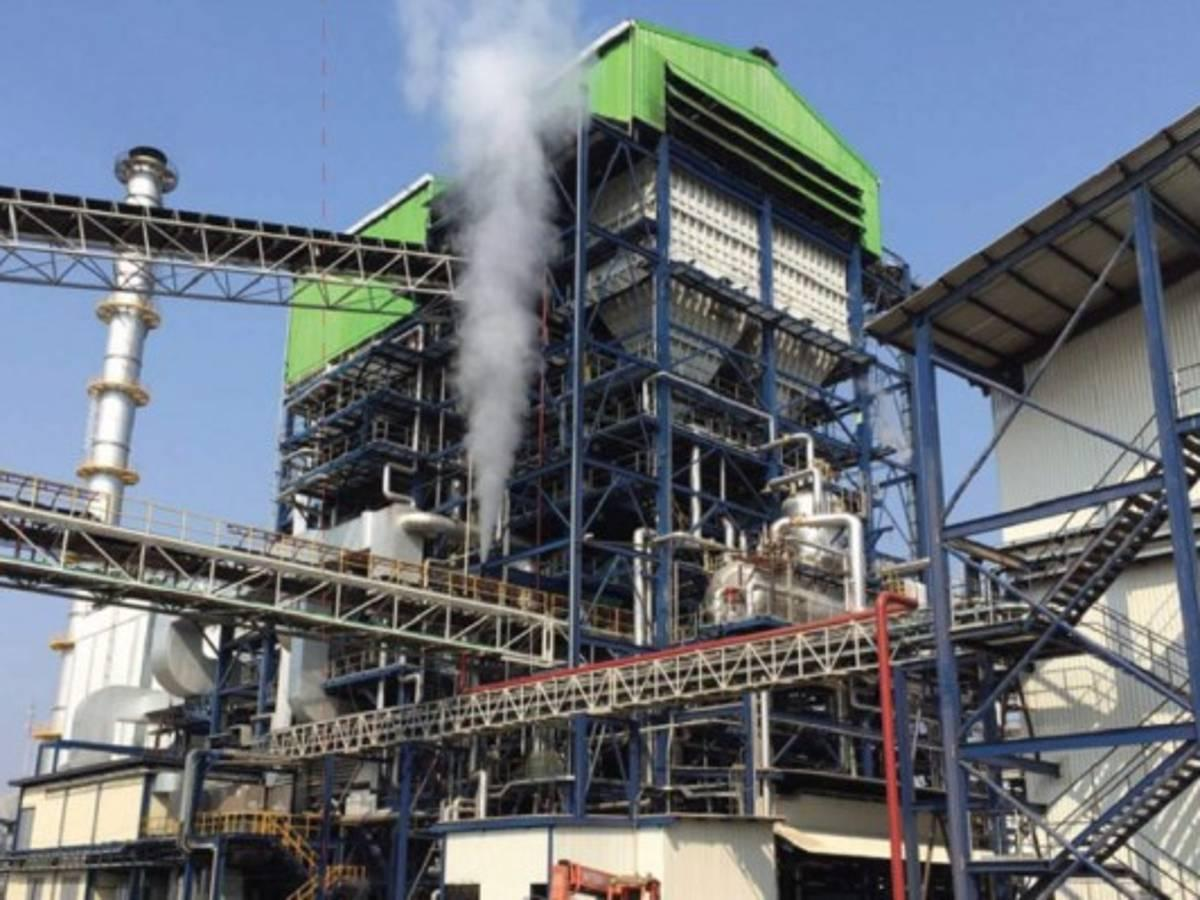
\includegraphics[width=0.9\textwidth]{Figuras/Sección C - Plantas de biomasa por el mundo/Planta de generación eléctrica del Ingenio Magdalena (Guatemala).jpg}
        \caption{Instalación industrial de generación eléctrica del Grupo Magdalena, en Guatemala. Se observan estructuras de calderas, tuberías, plataformas y equipos auxiliares empleados en la conversión térmica para producir electricidad. Es un ejemplo de infraestructura de generación energética vinculada a la industria azucarera guatemalteca}
    \end{figure}
\item \textbf{Gran escala --- Alholmens Kraft (Finlandia):} Considerada la mayor central de cogeneración con biomasa del mundo. Cuenta con $\sim 265~\mathrm{MW_e}$ instalados y una caldera de lecho fluidizado circulante (CFB) de $500~\mathrm{MW_{th}}$ a $165~\text{bar}$ y $545$~\textdegree C, suministrando además $100~\mathrm{MW_{th}}$ de vapor de proceso a una industria papelera vecina y $60~\mathrm{MW_{th}}$ de calefacción urbana a Pietarsaari \cite{alholmenskraft, flynn2005alholmens}. Fue diseñada como planta multicombustible (residuos forestales, turba y carbón); de sus 400 empleados, alrededor de 350 trabajan en la cadena de producción y manejo del combustible.
\item \textbf{Gran escala --- Drax Power Station (Reino Unido):} Originalmente la mayor central de carbón británica con seis unidades de $660~\text{MW}$. Entre 2013 y 2018 reconvirtió cuatro unidades para quemar exclusivamente pellets de madera ($\sim 2{,}6~\text{GW}$ totales), cerrando las dos unidades de carbón restantes en 2021 \cite{drax2025annual}. En 2024 generó más del 5~\% de la electricidad del Reino Unido, importando millones de toneladas anuales de pellets desde Norteamérica, lo que ilustra tanto la viabilidad de reutilizar infraestructura térmica como los límites logísticos de la gran escala.
\end{itemize}

\begin{figure}[H]
    \centering
    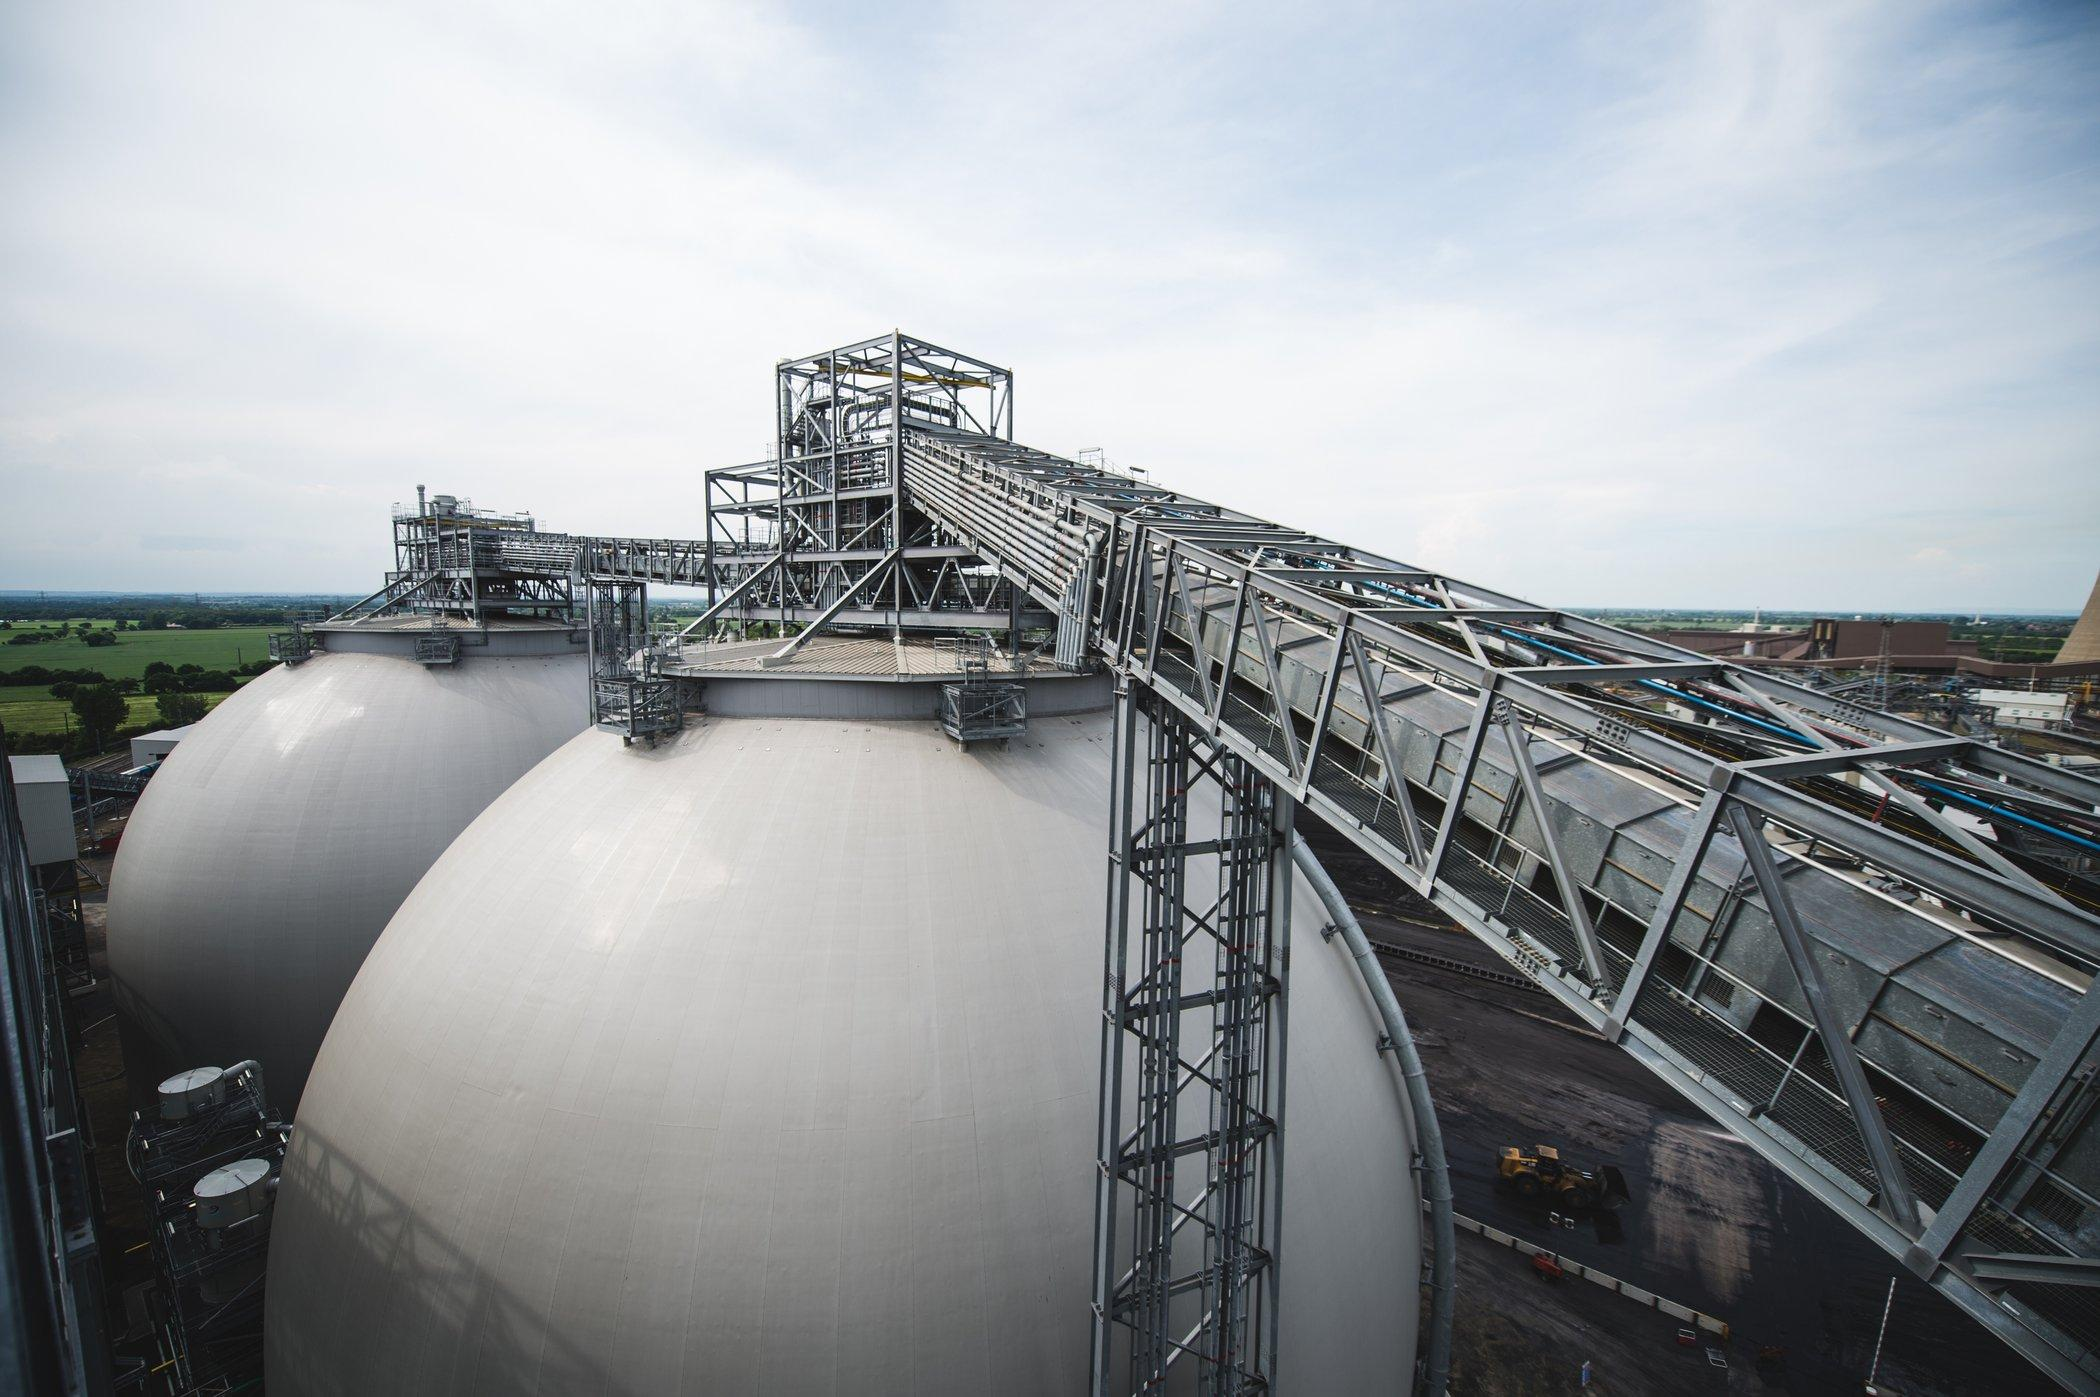
\includegraphics[width=0.75\textwidth]{Figuras/Sección C - Plantas de biomasa por el mundo/Sistema de almacenamiento de pellets de madera de Drax (Reino Unido).jpg}
    \caption{Grandes estructuras abovedadas utilizadas para almacenar pellets de madera en la central Drax. Estas instalaciones permiten mantener reservas de combustible para garantizar el suministro continuo a las unidades de generación, independientemente de las variaciones en las entregas de biomasa}
\end{figure}

\begin{figure}[H]
    \centering
    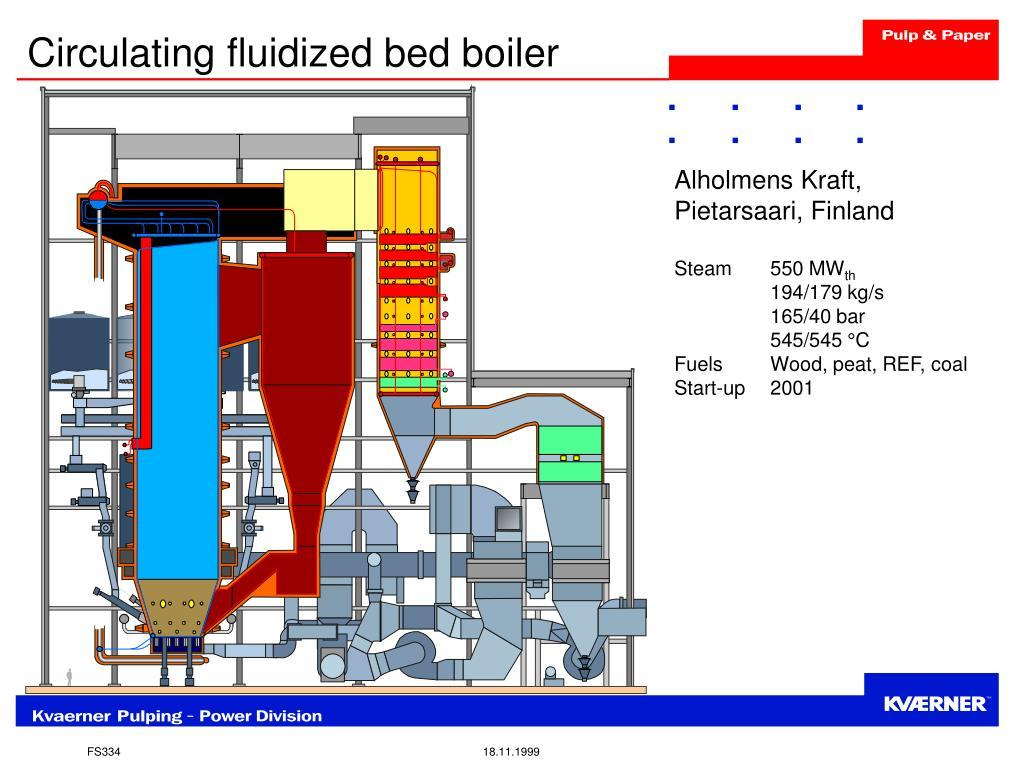
\includegraphics[width=0.7\textwidth]{Figuras/Sección C - Plantas de biomasa por el mundo/Caldera de lecho fluidizado circulante (CFB) de Alholmens Kraft.jpg}
    \caption{Esquema constructivo de una caldera de lecho fluidizado circulante utilizada en la central Alholmens Kraft, Finlandia. Se identifican la cámara de combustión, los sistemas de circulación de sólidos, los separadores ciclónicos y las superficies de intercambio térmico. Esta tecnología permite aprovechar diferentes combustibles sólidos y mantener condiciones de combustión controladas para producir vapor a alta presión y temperatura}
\end{figure}

\section{Configuraciones de planta}
\label{sec:configuraciones}

Según el aprovechamiento térmico y la integración con centrales existentes, se distinguen cuatro configuraciones principales (Tabla~\ref{tab:configuraciones_planta}). La \textbf{cogeneración (CHP)} es la configuración que mejor rentabiliza un combustible costoso de transportar, al elevar la eficiencia energética global al 70--90~\% mediante la venta o uso simultáneo de electricidad y vapor útil; esto exige ubicar la central junto al consumidor térmico (ingenios, papeleras, aserraderos o redes de distrito).

\begin{table}[htbp]
\centering
\caption{Configuraciones constructivas de centrales de biomasa.}
\label{tab:configuraciones_planta}
\begin{tabularx}{\textwidth}{@{}l X l l@{}}
\toprule
\textbf{Configuración} & \textbf{Descripción} & \textbf{Eficiencia típica} & \textbf{Ejemplo} \\
\midrule
Planta dedicada & Solo electricidad mediante turbina de condensación. & 20--35~\% eléctrica & Centrales forestales \\
Cogeneración (CHP) & Electricidad y calor útil del mismo combustible (contrapresión o extracción). & 70--90~\% global & Alholmens; ingenios \\
Co-combustión & Biomasa mezclada con carbón en caldera existente. & 36--44~\% eléctrica \cite{irena2013cofiring} & Centrales europeas \\
Conversión total & Central de carbón adaptada para operar 100~\% con biomasa. & Similar a la original & Drax \cite{drax2025annual} \\
\bottomrule
\end{tabularx}
\end{table}

\section{Aporte al sistema de potencia}
\label{sec:aporte_red}

A medida que crece la penetración de generación solar fotovoltaica y eólica ---recursos variables conectados a la red mediante inversores electrónicos---, los sistemas eléctricos demandan no solo energía, sino también potencia firme, flexibilidad operativa, inercia física y control de frecuencia y tensión \cite{bindu2025inertia, denholm2020inertia}. Una central de biomasa equipada con turbina y generador síncrono aporta estos servicios de estabilidad de manera natural, de forma equivalente a una central térmica convencional pero con combustible renovable.

\subsection{Potencia firme y reserva rodante}
Debido a que la biomasa se almacena en patios de astillas, silos de pellets o gasómetros, la generación puede programarse según la curva de demanda y no según la meteorología, explicando el factor de planta mundial medio de $\sim 53~\%$ \cite{wba2025gbsr}. En el Reino Unido, Drax suscribió un contrato por diferencia (CfD) como generación despachable baja en carbono a partir de abril de 2027 \cite{woodbioenergy2026drax}, y la IEA destaca el rol del biogás para el balance de red \cite{iea2025biogas}. La principal restricción es la estacionalidad de ciertos residuos agroindustriales como el bagazo.

En cuanto a la \textbf{reserva rodante}, las unidades sincronizadas que operan por debajo de su potencia nominal pueden incrementar carga ante la salida intempestiva de otro generador. En plantas de vapor, la velocidad de respuesta está limitada por la inercia térmica de la caldera (más lenta que en turbinas de gas o hidroeléctricas), mientras que los motogeneradores a biogás responden en minutos.

\subsection{Inercia rotacional y regulación primaria de frecuencia}
La inercia física corresponde a la energía cinética almacenada en las masas rotantes (turbina y rotor del generador síncrono) acopladas electromagnéticamente a la red \cite{nrel2014inertia, denholm2020inertia}. Ante la pérdida súbita de un generador ($\Delta P$), las masas rotantes liberan energía instantáneamente, frenando la caída de frecuencia y dando margen de actuación a los reguladores de velocidad. Se cuantifica mediante la constante de inercia $H$:
\begin{equation}
E_{\mathrm{cin}} = \frac{1}{2} J \omega^2, \qquad H = \frac{E_{\mathrm{cin}}}{S_n} \quad [\text{s}]
\end{equation}
donde $S_n$ es la potencia aparente nominal. La tasa inicial de cambio de frecuencia (\textit{Rate of Change of Frequency}, RoCoF) tras un desbalance $\Delta P$ resulta aproximadamente:
\begin{equation}
\frac{\mathrm{d}f}{\mathrm{d}t} \approx -\frac{\Delta P}{S_n} \cdot \frac{f_0}{2H}
\end{equation}
En un sistema de $60~\text{Hz}$ que pierde súbitamente el 5~\% de su generación ($\Delta P / S_n = 0{,}05$), con una inercia alta ($H = 4~\text{s}$) el RoCoF inicial es $\approx 0{,}38~\text{Hz/s}$; en cambio, en una red con alta penetración de inversores y baja inercia ($H = 2~\text{s}$), el RoCoF se duplica a $\approx 0{,}75~\text{Hz/s}$, pudiendo activar prematuramente los esquemas de deslastre de carga. Si bien los inversores modernos \textit{grid-forming} pueden emular inercia sintética, la inercia de los generadores síncronos de biomasa es intrínseca y madura.

Tras la respuesta inercial actúa la \textbf{regulación primaria}: el gobernador de la turbina ajusta la admisión de vapor según su estatismo $R$ (\textit{droop}, típicamente 4--5~\%):
\begin{equation}
\frac{\Delta P}{P_n} = -\frac{\Delta f / f_0}{R}
\end{equation}
Así, una unidad de biomasa de $30~\text{MW}$ con $R = 5~\%$ ($0{,}05$) ante una caída de frecuencia de $0{,}3~\text{Hz}$ ($0{,}5~\%$ de $60~\text{Hz}$) incrementa su potencia en $\Delta P = (0{,}005 / 0{,}05) \times 30~\text{MW} = 3~\text{MW}$. Posteriormente intervienen la regulación secundaria (AGC, en minutos) y la terciaria (redespacho).

\subsection{Control de tensión, potencia reactiva y filosofía de control}
Mediante su sistema de excitación y regulador automático de tensión (AVR), el generador síncrono inyecta o absorbe potencia reactiva dentro de su curva de capabilidad, sosteniendo el perfil de tensión en el punto de conexión. Esto resulta especialmente valioso porque muchas centrales de biomasa (ingenios, aserraderos) se ubican en zonas rurales al final de líneas largas de distribución o subtransmisión, donde la red es débil. Adicionalmente, aportan corriente de cortocircuito necesaria para la coordinación de protecciones.

Operativamente, las calderas de parrilla y lecho fluidizado presentan cargas mínimas técnicas del 30--50~\% nominal, rampas de pocos puntos porcentuales por minuto y arranques en frío de varias horas; los lechos fluidizados ofrecen una respuesta más suave por su gran masa térmica de arena. En el control de la central se distinguen dos filosofías: en el modo \textit{turbina sigue a caldera}, la válvula de admisión regula presión y la potencia sigue lentamente a la combustión (estable pero lento); en el modo \textit{caldera sigue a turbina}, la válvula responde de inmediato a la demanda aprovechando el vapor almacenado en el domo, permitiendo cumplir con la regulación primaria. Las centrales modernas emplean un control coordinado que combina ambos esquemas.

\begin{figure}[H]
    \centering
    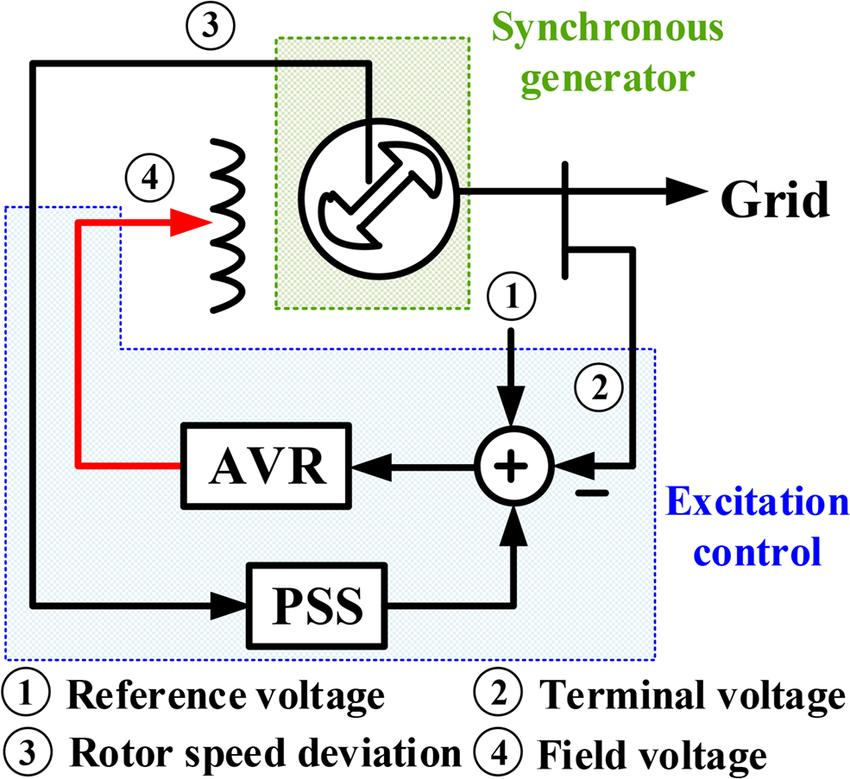
\includegraphics[width=0.98\textwidth]{Figuras/Sección C - Plantas de biomasa por el mundo/Sistema de excitación y regulación de tensión de un generador síncrono (AVR).jpg}
    \caption{Diagrama funcional del sistema de excitación de un generador síncrono, en el que se representa el regulador automático de tensión (AVR) y el estabilizador del sistema de potencia (PSS). El AVR compara la tensión de referencia con la tensión terminal del generador y ajusta la corriente de excitación para mantener el nivel de tensión requerido. El PSS contribuye a amortiguar las oscilaciones electromecánicas y mejorar la estabilidad del sistema eléctrico}
\end{figure}